\section{Esperança matemática}

\begin{synonyms}
    valor esperado, esperança, média.
\end{synonyms}

Se $X$ é uma \va\ discreta com valores no conjunto $A$
(finito ou infinito enumerável), a média de $X$ é
definida como

\begin{align}
    \Expected(X) &= \sum_{x \in A} x\cdot\Prob(X=x)
    \label{eq:ch02-esperança-discreta}
\end{align}

Se $X$ é uma \va\ contínua com com função densidade $f(x)$,
a média de $X$ é definida como

\begin{align}
    \Expected(X) &= \int_{-\infty}^{+\infty} x\cdot f(X=x) \wrt x
    \label{eq:ch02-esperança-continua}
\end{align}

\begin{obs}
    $\Expected(X)$ é definida se $\Expected(X) \in \R$.

    Pode acontecer que
    \begin{align*}
        \int_{-\infty}^{0} x\cdot f(X=x) &= -\infty
    \end{align*}
    e
    \begin{align*}
        \int_{+\infty}^{0} x\cdot f(X=x) &= +\infty
    \end{align*}
    Neste caso,
    \begin{align*}
        \Expected(X) &= \int_{-\infty}^{+\infty} x\cdot f(X=x) \\
        &= -\infty +\infty
    \end{align*}
    que é uma indeterminação. Logo, $\Expected(X)$ não existe.
\end{obs}

\begin{example}
    Uma loteria tem 100 bilhetes. O preço de um bilhete
    é R$\$ 1.20$. O bilhete sorteado paga um prêmio de
    R$\$ 100.00$. Você compra um bilhete. Qual é
    o seu ganho médio?

    \bigskip
    A \va\ $X$ representa o ganho:
    \begin{align*}
        X &= \begin{cases}
            0.00 - 1.20 &= -1.20,\ \text{se não ganhou}, \\
            100.00 - 1.20 &= 98.80,\ \text{se ganhou},
        \end{cases}
    \end{align*}
    com probabilidades
    \begin{align*}
        \Prob(X = -1.20) &= \frac{99}{100} \\
        \Prob(X = 98.80) &= \frac{1}{100}
    \end{align*}

    O ganho médio é
    \begin{align*}
        \Expected(X)
        &= -1.20 \cdot \Prob(X = -1.20)
            + 98.80 \cdot \Prob(X = 98.80) \\
        &= -1.20 \cdot \frac{99}{100}
            + 98.80 \cdot \frac{1}{100} \\
        &= -\text{R}\$ 0.20
    \end{align*}
\end{example}

\begin{example}[Interpretação física]
    A média $\Expected(X)$ é a posição de equilíbrio
    da distribuição de probabilidade.
    \begin{center}
        \begin{tikzpicture}
            \begin{axis}[
                unbounded coords=jump,
                grid=major,
                axis x line=middle,
                axis y line=middle,
                xmin=-6, xmax=12,
                ymin=0, ymax=0.45,
                xtick={4},
                xticklabels={$\Expected(X)$},
                ytick=\empty,
                extra tick style={grid=none},
                extra x ticks={-4, 2, 6, 10},
                extra x tick labels={
                    $x_1$,$x_2$,$x_3$,$x_4$
                },
                xlabel={$x$},
                ylabel={$\Prob(X = x)$},
                y label style={anchor=south},
                x label style={anchor=west},
            ]
            
            \addplot+[
                ycomb,
                dashed,
                blue]
                coordinates {
                    (-4, 1/9)
                    (2, 3.5/9)
                    (6, 3/9)
                    (10, 1.5/9)
                };

            \addplot[
                only marks,
                black]
                coordinates {
                    (4, 0)
                };

            \end{axis}
        \end{tikzpicture}
    \end{center}
    \begin{align*}
        \Expected(X) &= \sum_{i = 1}^4 x_i\cdot\Prob(X=x_i)
    \end{align*}
\end{example}

\begin{example}
    Considere
    \begin{align*}
        f(x) &= \begin{cases}
            2\exp(-2x) &,\ \text{se }x > 0, \\
            0          &,\ \text{caso contrário}.
        \end{cases}
    \end{align*}
    
    \begin{enumerate}[label=(\alph*)]
        \item\label{it:ch-02-exp-media-fdp}
        Prove que \begin{align*}
            \int_{-\infty}^{+\infty} f(x) \wrt x
            &= \int_0^{+\infty} f(x) \wrt x = 1.
        \end{align*}
    \end{enumerate}

    \bigskip
    \begin{proof}
        Calculamos
        \begin{align*}
            \int_{-\infty}^{+\infty} f(x) \wrt x
            &= \int_{-\infty}^{0} f(x) \wrt x
                + \int_{0}^{+\infty} f(x) \wrt x \\
            &= \cancelto{0}{\int_{-\infty}^{0} 0 \wrt x}
                + \int_{0}^{+\infty} 2\exp(-2x) \wrt x \\
            &= 2 \int_{0}^{+\infty} \exp(-2x) \wrt x \\
            &\phantom{===}
                \detail{u = -2x} \\
            &\phantom{===}
                \detail{\implies \wrt u = -2 \wrt x} \\
            &\phantom{===}
                \detail{\therefore -\frac{1}{2}\wrt u = \wrt x} \\
            &\phantom{===}
                \detail{x \to 0 \implies u \to 0} \\
            &\phantom{===}
                \detail{x \to +\infty \implies u \to -\infty} \\
            &= 2 \cdot \int_{0}^{-\infty}
                \exp(u) \cdot 
                \left(-\frac{1}{2}\right)
                \wrt u \\
            &= \cancel{2} \cdot \left(-\frac{1}{\cancel{2}}\right)
                \cdot \int_{0}^{-\infty}
                \exp(u)
                \wrt u \\
            &= -\left[\exp(u)
                \phantom{\frac{}{}}
                \right]_{u=0}^{u=-\infty} \\
            &= -\left[0 - 1\right] = 1
        \end{align*}
        pois $\lim_{u \to -\infty} \exp(u) = 0$ e $\exp(0) = 1$.
    \end{proof}

    \begin{enumerate}[label=(\alph*)]
        \item Calcule $\Expected(X)$.
    \end{enumerate}

    Calculamos
    \begin{align*}
        \int_{-\infty}^{+\infty} x\cdot f(x) \wrt x
        &= \int_{-\infty}^{0} x\cdot f(x) \wrt x
            + \int_{0}^{+\infty} x\cdot f(x) \wrt x \\
        &= \cancelto{0}{\int_{-\infty}^{0} 0 \wrt x}
            + \int_{0}^{+\infty} x\cdot 2\exp(-2x) \wrt x \\
        &= 2 \int_{0}^{+\infty} x\cdot \exp(-2x) \wrt x \\
        &\phantom{===}
            \detail{\int u\wrt v = uv -  \int v\wrt u} \\
        &\phantom{===}
            \detail{u = x \implies \wrt u = \wrt x} \\
        &\phantom{===}
            \detail{\wrt v = \exp(-2x) \wrt x
                \implies v = -\frac{1}{2} \exp(-2x)} \\
        &= 2\cdot \left\{
            \cancelto{0}{\left[
                x\cdot\left(-\frac{1}{2}\right) \exp(-2x)
            \right]_{x=0}^{+\infty}} \right. \\
        &\phantom{2\cdot =}\left.
            - \int_{0}^{+\infty}
                \left(-\frac{1}{2}\right) \exp(-2x) \wrt x
        \right\} \\
        &= -\left(-\frac{1}{2}\right)
            \underbrace{\int_{0}^{+\infty} \exp(-2x) \wrt x}
            _{= 1\ (\text{pelo \cref{it:ch-02-exp-media-fdp}})} \\
        &= \frac{1}{2}
    \end{align*}

    \begin{center}
        \begin{tikzpicture}
            \begin{axis}[
                unbounded coords=jump,
                grid=major,
                axis x line=middle,
                axis y line=middle,
                xmin=-.2, xmax=1.2,
                ymin=0, ymax=2.1,
                xtick={1/4,1/3,1/2,1},
                xticklabels={
                    $\sfrac{1}{4}$,
                    $\sfrac{1}{3}$,
                    $\sfrac{1}{2}$,
                    1
                },
                ytick={2, 1.2131, 1.0268, 0.7358, 0.2707},
                xlabel={$x$},
                ylabel={$f(x)$},
                y label style={anchor=south},
                x label style={anchor=west},
            ]
            
            \addplot[ultra thick, blue, domain=0:2, samples=100]
                {2*exp(-2*x)};

            \addplot[ultra thick, blue, domain=-.5:0, samples=2]
                {0};

            \addplot[blue, fill=white, only marks, ultra thick,
                samples at={0}] {2};

            \addplot[blue, only marks, ultra thick,     
                samples at={0}] {0};

            \end{axis}
        \end{tikzpicture}
    \end{center}
\end{example}

\begin{example}
    Considere a \va\ $X$, cuja distribuição é dada pelo gráfico abaixo.

    Devido à simetria da distribuição, espera-se que
    a média esteja no ponto de simetria. De fato, 
    para esta distribuição, $\Expected(X) = a$.

    \begin{obs}
        Há distribuições que, apesar de serem simétricas,
        elas não têm média.
    \end{obs}
    
    \begin{center}
        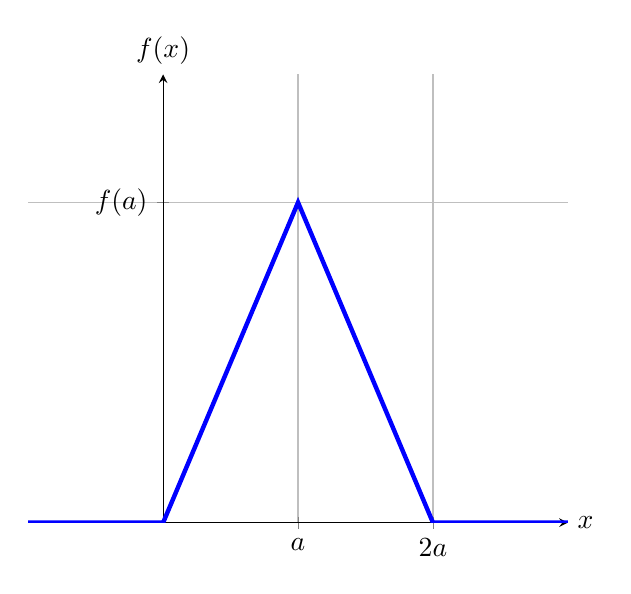
\begin{tikzpicture}
            \begin{axis}[
                unbounded coords=jump,
                grid=major,
                axis x line=middle,
                axis y line=middle,
                xmin=-.5, xmax=1.5,
                ymin=0, ymax=.7,
                xtick={1/2,1},
                xticklabels={$a$, $2a$},
                ytick={1/2},
                yticklabels={$f(a)$},
                xlabel={$x$},
                ylabel={$f(x)$},
                y label style={anchor=south},
                x label style={anchor=west},
            ]
            
            \addplot[ultra thick, blue]
                coordinates {
                    (-1, 0)
                    (0, 0)
                    (.5, .5)
                    (1, 0)
                    (2, 0)
                };

            \end{axis}
        \end{tikzpicture}
    \end{center}
\end{example}
